\section{Feature Extraktion bei kontinuierlichen Livedaten}\label{kap:featureextraktion}

Die Sensordaten zur Überwachung von Maschinen erzeugen einen kontinuierlichen Datenfluss. Wie in den voherigen Kaptiteln beschrieben, stellt diese Eigenschaft eine hohe Anforderung an Lernalgorithmen. Einige Lernalgorithmen verwenden das Konzept des \enquote{Lazy Learnings}, im Deutschen \enquote{träges Lernen}. Bei diesen Lernalgorithmen wird das Modell auf Anfrage erstellt. Das bedeutet, jede Eingabe startet eine neue Modellbildung und fordet daher in kürzester Zeit eine hohe Rechenleistungen. Beim \enquote{Eeager Learning}, im Deutschen \enquote{Eifriges Lernen}, hingegen wird schon im Vorfeld mithilfe von Trainingsdaten ein Model bereitgestellt. Der Ressourcenverbrauch bei einer Anfrage von neuen Daten ist dann sehr gering~\cite{Gay2013}. 

Bei den kontinuierlichen Livedaten in der Maschinenüberwachung stehen die Daten meist auch zeitlich in korrelation. Daher ist die Rede von Zeitreihen Daten. Die Reihenfolge dieser Daten spielt bei der Analyse eine große Rolle. Zeitreihendatensätze werden mathematisch wie in dem Datensatz \ref{equ:trainingset} dargestellt. Eines der Ziele für Lernalgorithmen kann es sein aus dem Datensatz \ref{equ:trainingset} die Daten 

\begin{equation}
  \tau_{n+1}, \tau_{n+2}, ...
  \label{equ:predictionset}
\end{equation}
voherzusagen.

Um die Komplexität der Zeitreihendatensätze zu reduzieren wird die Dimension, entstehend durch die Parameter, versucht möglichst auf die notwendigen Merkmale zu reduzieren. Zeitreihendaten aus Sensoren sind oft hoch korrelierend, was zu einer sehr großen Datenredunanz führt. 
Eine bewerte Technik um Datenmengen aus Sensordaten fester größe darzustellen ist die \enquote{Fourier Transforamtion}. Dabei werden die Signale auf einen Frequenzbereich abgebildet und diese Abbildung mittels Koeffizienten dargestellt. Da es sich bei den kontinuierlichen Sensordaten meist um keinen vollständigen Datenbestand handelt, sondern nur Datenauszüge bietet sich die \enquote{Diskrete Fourier Transformation} an.

\begin{equation}
  F_j = \frac{1}{N} \sum_{k=0}^{N-1} f_k W_N^{-kj}  \text{\ \ mit \ \ } W_N = e^{\frac{2\pi i}{N}}
  \label{equ:fourier}
\end{equation}

Durch die Diskrete Fourier Transformation in Formel\ \ref{equ:fourier} wird der Zeitreihenabschnitt in einer periodische Funktion durch Koeffizienten dargestellt~\cite{Butz2012}. Um die zu analysierdenen Merkmale zu reduzieren ist die Idee,dass nicht alle Koeefizienten als Parameter verwenden werden, sondern nur eine Auswahl von diesen. Bekannte Methoden sind dabei entweder die ersten $k$ Koeffizienten zu verwenden. Man speichert quasi nur eine grobe Skizze der Kurven ab. Die ersten Koeffizienten abzuspeichern, behält die tieferen Frequenzen und ist eine sehr naive herangehensweise. Eine deutlich bessere Methode wäre es die größten Koeffizienten zu verwenden. Diese sind aber sehr aufwändig zu berechnen~\cite{morchen2003time}. Fabian Mörchen stellt dagegen eine Methode in seiner Arbeit \enquote{Time series feature extraction for data mining using DWT and DFT} vor, in der er eine Aggregatsfunktion verwendet, welche die Bedeutung der Koeffizienten misst. Es ist dadurch möglich mit seiner Aggregatsfunktion:

\begin{equation}
  J_k^1(mean(c_j^2), C)
  \label{equ:aggregatefunction}
\end{equation}

eine definierte Menge $k$ an Koeffizienten als Merkmale für Lernalgorithmen als Eingabe zu geben. $k$ entspricht dann der Dimension der zu verarbeitenden Datenmenge. 

Eine weitere Arbeit von Dominique Gay et al. \enquote{Feature Extraction over Multiple Representations for Time Series Calssification} stellt ein Verfahren vor in dem sie Zeitreihendaten so vorverarbeiten, dass in dem Verfahren extrahierte Merkmale die neuen Parameter fester Größe bilden. Dies geschieht in einem drei Schritteverfahren:

\begin{enumerate}
  \item Der Datensatz wird in mehrere Datenrepräsentationen transformiert
  \item Auf jede Repräsentation wird ein Co-Clustering Verfahren angewendet
  \item Aus jeder Repräsentation wird eine Menge an Merkmalen erstellt und daraus ein neuer Datensatz generiert
\end{enumerate}

Für den ersten Schritt schlagen sie verschiedene Transformationsverfahren vor. Beispielsweise Ableitungen oder comulatives Integrieren. In einem Beispiel sind die Vorteile einer solchen Vorverarbeitung erkennbar. In Abbildung\ \ref{fig:derivative} ist in (a) ein zwei Klassen ARSim Datensatz zu sehen. Dieser ist unverarbeitet und die Klassen sind farblich Markiert. Die Klassen sind in (a) nur sehr schwer separierbar. In (b) wurde der selbe Datensatz durch zweifaches Ableiten transformiert und wieder in einem Datenplot und farblicher markierung dargetsellt. Durch die Transformation sind die Klassen schon deutlicher erkennbar.

\begin{figure}
  \centering
  \includegraphics[width=1\textwidth]{plotAbleitung.png}
  \caption{In (a) ein unverarbeiteter original geplotteter Datensatz und in (b) der gleiche durch zweifache Ablteiungen transformierter Datensatz~\cite{Gay2013}.}
  \label{fig:derivative}
\end{figure}

Der transformierte Datensatz bilde somit eine bessere Grundlage um mithilfe von Klassifizierungsalgorithmen die Daten zu Differenzieren. 
Der zweite Schritt ist das Co-Clustering. 
Dabei wird das Clustering als eine Vorverarbeitung für nachfolgende Lernalgorithmen verwendet. 
Die Idee ist es ähnliche Daten zu gruppieren und lokale Muster hervorzuheben~\cite{gay2013feature}. Dabei stellen sie die Kurven in einer Menge $(X,Y)$ dar und fügen jeder dieser Mengen eine Klasse $Cid$ hinzu um sie der jeweiligen Kurve zuzuordnen. Es entsteht eine dreidimensinale Darstellung der Punkte. Das Ganze wird in eine dreidimensionale Gitterstruktur gebracht. Das Endziel ist es Kurven- und Intervallcluster zu erhalten die Anschließend als Merkmalsgrundlage dienen. 

Erreicht wird das durch das Anwenden des \enquote{Khiops Coclustering}\cite{boulle2012functional}. Dabei wird das optimale Gitterfeld durch die Optimierung des Bayes'schen Kriteriums, der sogenannen Kosten ermittelt. 
\begin{equation}
  cost(M) = -log(p(M) \times p(D|M))
  \label{equ:Bayesian}
\end{equation}
Als resultat lassen sich die Kosten so interpretieren, dass bei niedrigen Kosten eine hohe Kompression der Daten $D$ auf das Modell $M$ herrscht. Wobei das Modell in diesem Fall das optimale Gitterfeld ist.

\begin{figure}
  \centering
  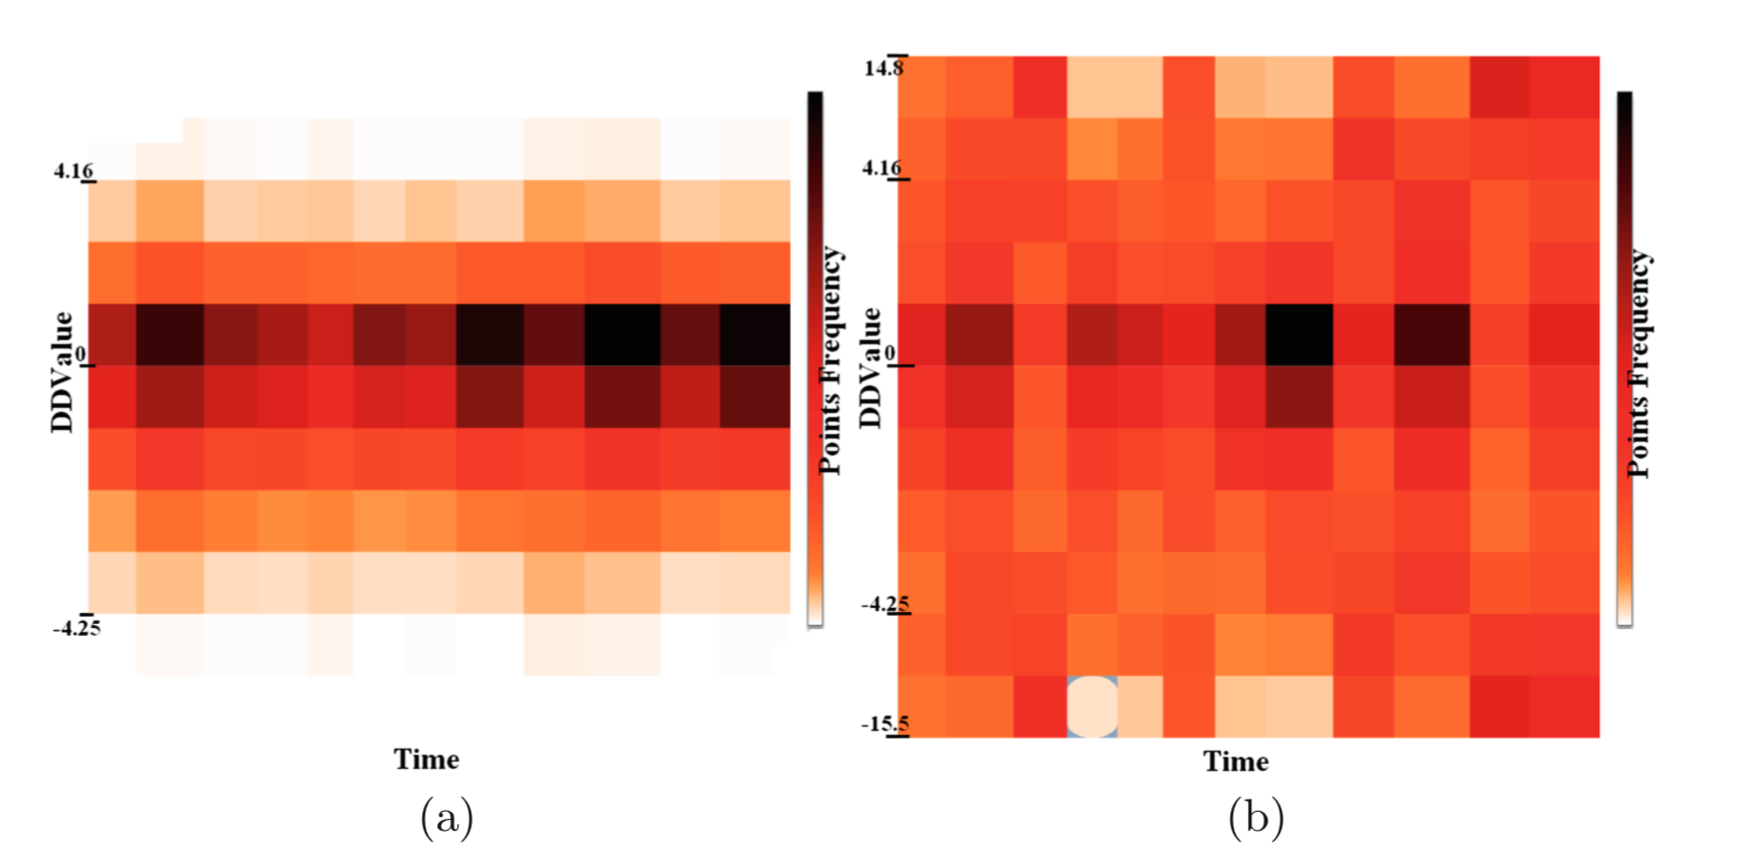
\includegraphics[width=1\textwidth]{coclustering.png}
  \caption{Ergebniss eines CoCluserings mit Khiops Coclustering~\cite{Gay2013}.}
  \label{fig:coclustering}
\end{figure}

Ein durchgeführtes Co-Clustering ist in Abbildung\ \ref{fig:coclustering} zu sehen. Dabei ist die dritte Dimension Farblich dargestellt. Als Ergebnis sind 25 Cluster von Kurven entstanden. 

Als letzten Schritten müssen noch die Merkmale extrahiert und ein Datensatz generiert werden. Es werden dre Merkmale definiert:

\begin{enumerate}
  \item $K_C$ ein numerisches Merkmal, welches die Unähnlichkeitswahrscheinlichkeit zu allen Kurvenclustern angibt.
  \item Ein kategorisches Merkmal als index, welcher das nächste Kurvencluster angibt.
  \item $K_Y$ ein nummerisches Merkmal, welches die Anzahl an Punkten dieser Kurve in der jeweiligen Klasse angibt.
\end{enumerate}

Durch dieses Verfahren wird die Dimension der Livedaten mit Hilfe von \enquote{Feature Extraktion} auf Drei festgelegt und kann somit durch \enquote{Eager Learning} Algorithmen analysiert werden.
